\iffalse
\documentclass[12pt]{article}
\usepackage{graphicx}
\usepackage{amsmath}
\usepackage{mathtools}
\usepackage{gensymb}

\newcommand{\mydet}[1]{\ensuremath{\begin{vmatrix}#1\end{vmatrix}}}
\providecommand{\brak}[1]{\ensuremath{\left(#1\right)}}
\providecommand{\norm}[1]{\left\lVert#1\right\rVert}
\newcommand{\solution}{\noindent \textbf{Solution: }}
\newcommand{\myvec}[1]{\ensuremath{\begin{pmatrix}#1\end{pmatrix}}}
\let\vec\mathbf

\begin{document}
\begin{center}
\section*{CHAPTER 7 - COORDINATE GEOMETRY}

\end{center}
\section*{Excercise 7.1}

Q4.Check whether (5,-2),(6,4) and (7,-2) are the vertices of an isosceles triangle:

\solution
\fi
Let us assume the given three points to be
	\begin{align}
		\vec{A} = \myvec{5 \\-2},\vec{B}= \myvec{6\\4}, \vec{C} = \myvec{7\\-2}.
	\end{align}
Forming the matrix
	\begin{align}
\vec{P} = \myvec{
5&6&7\\
-2&4&-2
}\xrightarrow[]{R_2=\frac{R_2}{2}}
\myvec{
5&6&7\\
-1&2&-1
}\xrightarrow[]{R_1=\frac{R_1}{5}}
\myvec{
1&\frac{6}{5}&\frac{7}{5}\\
-1&2&-1
}\\\xrightarrow[]{R_2=R_2+R_1}
\myvec{
1&\frac{6}{5}&\frac{7}{5}\\
0&\frac{16}{5}&\frac{2}{5}
}\xrightarrow[]{R_2=\frac{R_2}{16/5}}
\myvec{
1&\frac{6}{5}&\frac{7}{5}\\
0&1&\frac{1}{8}
}
	\end{align}
$\text{rank}(P) = 2$ and the given points form a triangle. Since
	\begin{align}
		\vec{A}-\vec{B} &= \myvec{5\\-2} - \myvec{6\\4} &= \myvec{-1\\-6} \\
		\vec{B}-\vec{C} &= \myvec{6\\4} - \myvec{7\\-2} &= \myvec{-1\\6} \\
		\vec{C}-\vec{A} &= \myvec{7\\-2} - \myvec{5\\2} &= \myvec{2\\0},
		\norm{\vec{A}-\vec{B}} &=
\norm{\vec{B}-\vec{C}}  = \sqrt{37} 
	\end{align}
	Thus, the triangle is isosceles.  See Fig. 
\ref{fig:chapters/10/7/1/4/Fig}.
\begin{figure}[H]
	\begin{center} 
	    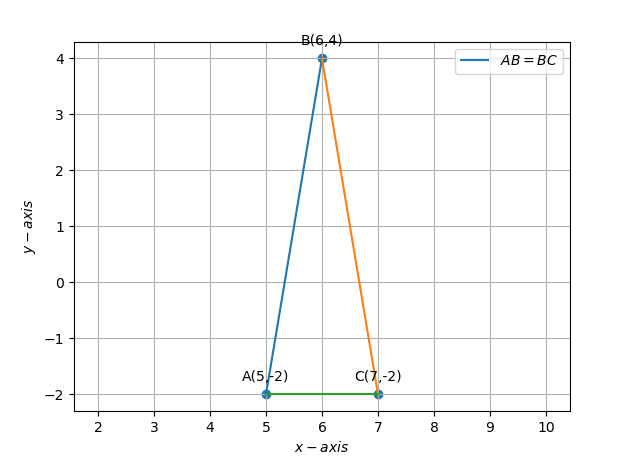
\includegraphics[width=0.75\columnwidth]{chapters/10/7/1/4/figs/Vector2.png}
	\end{center}
\caption{}
\label{fig:chapters/10/7/1/4/Fig}
\end{figure}
